\begin{center}
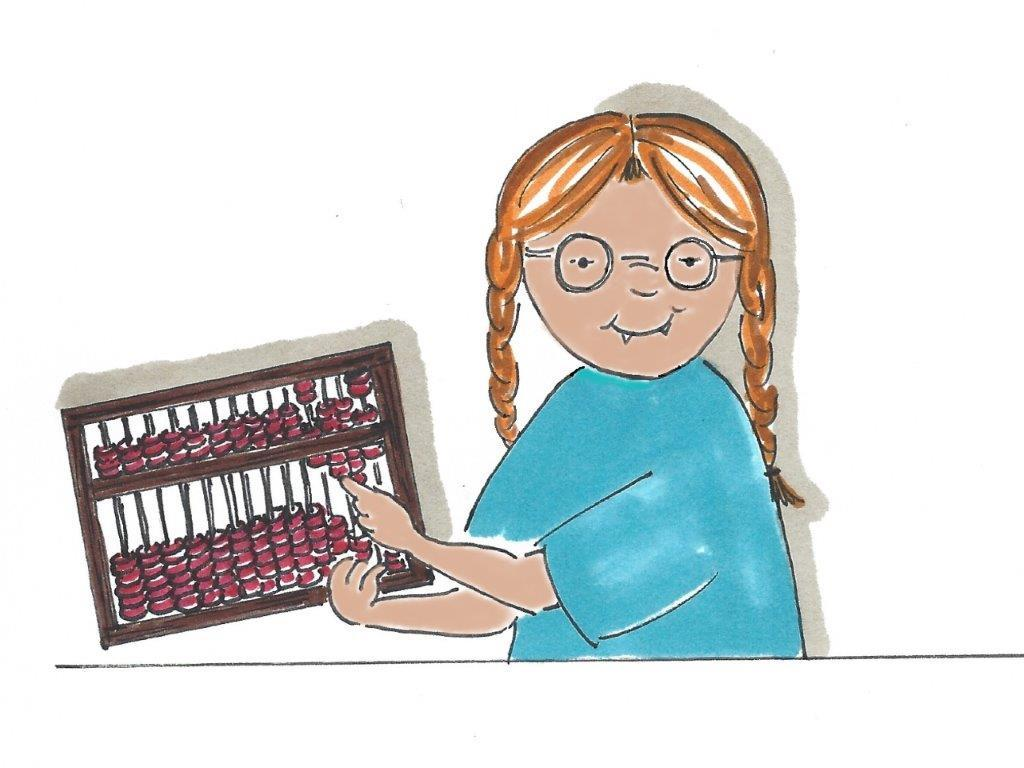
\includegraphics[width=0.6\textwidth]{content/3/chapter5/images/15.png}\\
Cippi studies arithmetic
\end{center}

The comparison of signed and unsigned integers is a subtle cause for unexpected behavior and, therefore, of bugs. Thanks to the new safe comparison functions for integers, std::cmp\_*, a source of subtle bugs is gone. Additionally, C++20 includes mathematical constants such as e, π, or ϕ, and with the functions std::midpoint and std::lerp, you can calculate the midpoint of two numbers or their linear interpolation. The new bit manipulation allows you to access and modify individual bits or bit sequences.

\subsubsubsection{5.4.1\hspace{0.2cm} Safe Comparison of Integers}

When you compare signed and unsigned integers, you may not get the result you expect. Thanks to the six std::cmp\_* functions, there is a cure in C++20. To motivate safe comparison of integers, I want to start with the unsafe variant.

\begin{tcolorbox}[breakable,enhanced jigsaw,colback=blue!5!white,colframe=blue!75!black,title={Integral versus Integer}]
	
The terms integral and integer are synonyms in C++. This is the wording from the standard for fundamental types: “Types bool, char, char8\_t, char16\_t, char32\_t, wchar\_t, and the signed and unsigned integer types are collectively called integral types. A synonym for [an] integral type is integer type”. I prefer the term integer in this book.
	
\end{tcolorbox}

\noindent
5.4.1.1\hspace{0.2cm} Unsafe Comparison

Of course, there is a reason for the name unsafeComparison.cpp of the following program.

\noindent
Unsafe comparison of integers
\begin{lstlisting}[style=styleCXX]
// unsafeComparison.cpp

#include <iostream>

int main() {
	
	std::cout << '\n';
	
	std::cout << std::boolalpha;
	
	int x = -3;
	unsigned int y = 7;
	
	std::cout << "-3 < 7: " << (x < y) << '\n';
	std::cout << "-3 <= 7: " << (x <= y) << '\n';
	std::cout << "-3 > 7: " << (x > y) << '\n';
	std::cout << "-3 => 7: " << (x >= y) << '\n';
	
	std::cout << '\n';

}
\end{lstlisting}

When I execute the program, the output may not meet your expectations.

\begin{center}
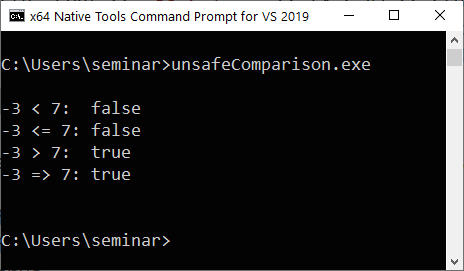
\includegraphics[width=0.6\textwidth]{content/3/chapter5/images/16.png}\\
Surprises with unsafe comparisons of integers
\end{center}

When you read the output of the program, you recognize that -3 is bigger than 7. You presumably know the reason. I compared a signed x (line 11) with an unsigned y (line 12). What is happening under the hood? The following program provides the answer.

\noindent
Unsafe comparison of integers resolved
\begin{lstlisting}[style=styleCXX]
// unsafeComparison2.cpp

int main() {
	int x = -3;
	unsigned int y = 7;
	
	bool val = x < y;
	static_assert(static_cast<unsigned int>(-3) == 4'294'967'293);
}
\end{lstlisting}

In the example, I’m focusing on the less-than operator. \href{https://cppinsights.io/s/62732a01}{C++ Insights} gives me the following output:

\begin{center}
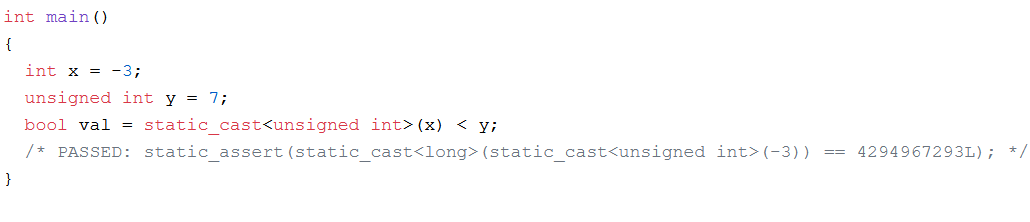
\includegraphics[width=0.6\textwidth]{content/3/chapter5/images/1-4.png}\\
Unsafe comparison analyzed
\end{center}

Here is what’s happening:

\begin{itemize}
\item 
The compiler transforms the expression x < y (line 7) into static\_cast<unsigned int>(x) < y. In particular, the signed x is converted to an unsigned int.

\item 
Due to the conversion, -3 becomes 4'294'967'293.

\item 
4'294'967'293 is equal to −3 mod $ 2^{32} $

\item 
32 is the number of bits of an unsigned int on C++ Insights.
\end{itemize}

Thanks to C++20, we have a safe comparison of integers.

\hspace*{\fill} \\ %插入空行
\noindent
\textbf{5.4.1.2\hspace{0.2cm} Safe Comparison of Integers}

C++20 supports six comparison functions for integers:

\begin{center}
Six safe comparison functions
\end{center}

\begin{table}[H]
\centering
\begin{tabular}{ll}
\textbf{compare Function} & \textbf{Meaning} \\ \hline
std::cmp\_equal           & ==               \\
std::cmp\_not\_equal      & !=               \\
std::cmp\_less            & \textless{}      \\
std::cmp\_less\_equal     & \textless{}=     \\
std::cmp\_greater         & \textgreater{}   \\
std::cmp\_greater\_equal  & \textgreater{}= 
\end{tabular}
\end{table}

Thanks to the six comparison functions, I can easily transform the previous program unsafeComparison.cpp into the program safeComparison.cpp. The new comparison functions require the header <utility>.

\noindent
Safe comparison of integers
\begin{lstlisting}[style=styleCXX]
// safeComparison.cpp

#include <iostream>
#include <utility>

int main() {
	
	std::cout << '\n';
	
	std::cout << std::boolalpha;
	
	int x = -3;
	unsigned int y = 7;
	
	std::cout << "-3 == 7: " << std::cmp_equal(x, y) << '\n';
	std::cout << "-3 != 7: " << std::cmp_not_equal(x, y) << '\n';
	std::cout << "-3 < 7: " << std::cmp_less(x, y) << '\n';
	std::cout << "-3 <= 7: " << std::cmp_less_equal(x, y) << '\n';
	std::cout << "-3 > 7: " << std::cmp_greater(x, y) << '\n';
	std::cout << "-3 => 7: " << std::cmp_greater_equal(x, y) << '\n';
	
	std::cout << '\n';
	
}
\end{lstlisting}

Additionally, I applied the equal and not equal operators.

\begin{tcblisting}{breakable,commandshell={}}
-3 == 7: false
-3 != 7: true
-3 < 7: true
-3 <= 7: true
-3 > 7: false
-3 => 7: false
\end{tcblisting}

\begin{center}
Safe comparison
\end{center}

Invoking a safe-comparison function with a non-integer, such as a double, causes a compile-time error.

\noindent
Safe comparison of an unsigned int and a double
\begin{lstlisting}[style=styleCXX]
// safeComparison2.cpp

#include <iostream>
#include <utility>

int main() {
	
	double x = -3.5;
	unsigned int y = 7;
	
	std::cout << "-3.5 < 7: " << std::cmp_less(x, y); // ERROR
	
}
\end{lstlisting}

On the other hand, you can compare a double and an unsigned int the classical way. The program classicalComparison.cpp applies classical comparison of a double and an unsigned int.

\noindent
Classical comparison of an unsigned int and a double
\begin{lstlisting}[style=styleCXX]
// classicalComparison.cpp

int main() {
	
	double x = -3.5;
	unsigned int y = 7;
	
	auto res = x < y; // true
	
}
\end{lstlisting}

It works. The unsigned int is \href{https://en.cppreference.com/w/cpp/language/implicit_conversion}{floating-point promoted} to double. \href{https://cppinsights.io/s/44216566}{C++ Insights} shows the truth:

\begin{center}
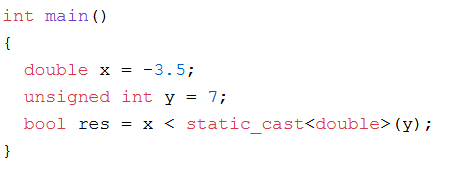
\includegraphics[width=0.6\textwidth]{content/3/chapter5/images/1-5.png}\\
Floating point promotion to double
\end{center}

\subsubsubsection{5.4.2\hspace{0.2cm} Mathematical Constants}

First of all, the constants require the header <numbers> and the namespace std::numbers. The following table gives you an overview.

\begin{center}
The mathematical constants
\end{center}

\begin{table}[H]
\centering
\begin{tabular}{ll}
Mathematical Constant     & Description               \\ \hline
std::numbers::e           & $e$                       \\
std::numbers::log2e       & $log_{2}e$                \\
std::numbers::log10e      & $log_{10}e$               \\
std::unmbers::pi          & $\pi$                     \\
std::unmbers::inv\_pi     & $\frac{1}{\pi}$           \\
std::numbers::inv\_sqrtpi & $\frac{1}{\sqrt{\pi}}$    \\
std::numbers::ln2         & ln2                       \\
std::numbers::ln10        & ln10                      \\
std::numbers::sqrt2       & $\sqrt{2}$                \\
std::numbers::sqrt3       & $\sqrt{3}$                \\
std::numbers::inv\_sqrt3  & $\frac{1}{\sqrt{3}}$      \\
std::numbers::egamma      & \href{https://en.wikipedia.org/wiki/Euler%E2%80%93Mascheroni_constant}{Euler-Mascheroni constant} \\
std::numbers::phi         & $\phi$                   
\end{tabular}
\end{table}

The program mathematicConstants.cpp applies the mathematical constants.

\noindent
The mathematical constants
\begin{lstlisting}[style=styleCXX]
// mathematicConstants.cpp

#include <iomanip>
#include <iostream>
#include <numbers>

int main() {
	std::cout << '\n';
	
	std::cout<< std::setprecision(10);
	
	std::cout << "std::numbers::e: " << std::numbers::e << '\n';
	std::cout << "std::numbers::log2e: " << std::numbers::log2e << '\n';
	std::cout << "std::numbers::log10e: " << std::numbers::log10e << '\n';
	std::cout << "std::numbers::pi: " << std::numbers::pi << '\n';
	std::cout << "std::numbers::inv_pi: " << std::numbers::inv_pi << '\n';
	std::cout << "std::numbers::inv_sqrtpi: " << std::numbers::inv_sqrtpi << '\n';
	std::cout << "std::numbers::ln2: " << std::numbers::ln2 << '\n';
	std::cout << "std::numbers::sqrt2: " << std::numbers::sqrt2 << '\n';
	std::cout << "std::numbers::sqrt3: " << std::numbers::sqrt3 << '\n';
	std::cout << "std::numbers::inv_sqrt3: " << std::numbers::inv_sqrt3 << '\n';
	std::cout << "std::numbers::egamma: " << std::numbers::egamma << '\n';
	std::cout << "std::numbers::phi: " << std::numbers::phi << '\n';
	
	std::cout << '\n';
}
\end{lstlisting}

Here is the output of the program with the MSVC compiler.

\begin{center}
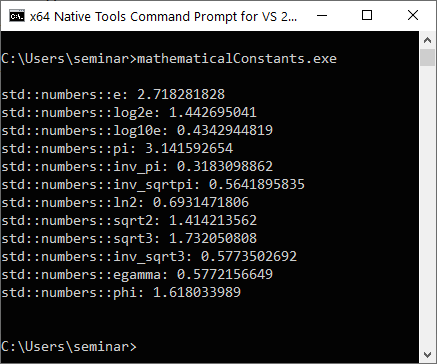
\includegraphics[width=0.6\textwidth]{content/3/chapter5/images/17.png}\\
Use of all mathematical constants
\end{center}

The mathematical constants are available for float, double, and long double. By default, double is used but, you can also specify float (std::numbers::pi\_v<float>) or long double (std::numbers::pi\_v<long double>).

\subsubsubsection{5.4.3\hspace{0.2cm} Midpoint and Linear Interpolation}

\begin{itemize}
\item 
std::midpoint(a, b): calculates the midpoint (a + (b - a) / 2) of integers, floating points, or pointers. If a and b are pointers, they have to point to the same array object. The function needs the header <numeric>.

\item 
std::lerp(a, b, t): calculates the linear interpolation (a + t(b - a)). When t is outside the range [0, 1], it calculates the linear extrapolation. The function needs the header <cmath>.
\end{itemize}

The program midpointLerp.cpp applies both functions.

\noindent
Calculating the midpoint and the linear interpolation of numbers
\begin{lstlisting}[style=styleCXX]
// midpointLerp.cpp

#include <cmath>
#include <numeric>
#include <iostream>

int main() {
	
	std::cout << '\n';
	
	std::cout << "std::midpoint(10, 20): " << std::midpoint(10, 20) << '\n';
	
	std::cout << '\n';
	
	for (auto v: {0.0, 0.1, 0.2, 0.3, 0.4, 0.5, 0.6, 0.7, 0.8, 0.9, 1.0}) {
		std::cout << "std::lerp(10, 20, " << v << "): " << std::lerp(10, 20, v)
				  << '\n';
	}
	
	std::cout << '\n';
	
}
\end{lstlisting}

The program should, together with its output, be self-explanatory.

\begin{tcblisting}{breakable,commandshell={}}
std::midpoint(10, 20): 15

std::midpoint(10, 20, 0): 10
std::midpoint(10, 20, 0.1): 11
std::midpoint(10, 20, 0.2): 12
std::midpoint(10, 20, 0.3): 13
std::midpoint(10, 20, 0.4): 14
std::midpoint(10, 20, 0.5): 15
std::midpoint(10, 20, 0.6): 16
std::midpoint(10, 20, 0.7): 17
std::midpoint(10, 20, 0.8): 18
std::midpoint(10, 20, 0.9): 19
std::midpoint(10, 20, 1): 20
\end{tcblisting}

\begin{center}
Calculating the midpoint and the linear interpolation of numbers
\end{center}

\subsubsubsection{5.4.4\hspace{0.2cm} Bit Manipulation}

The header <bit> supports functions to access and manipulate individual bits or bit sequences.

\hspace*{\fill} \\ %插入空行
\noindent
\textbf{5.4.4.1\hspace{0.2cm} std::endian}

Thanks to the new type std::endian, you get the endianness of a scalar type. Endianness can be bigendian or little-endian. Big-endian means that the most significant byte is furthest left, little-endian means that the least significant byte is furthest left. A scalar type is either an arithmetic type, an enum, a pointer, a member pointer, or a std::nullptr\_t.

The class endian provides the endianness of all scalar types:

\noindent
enum class endian
\begin{lstlisting}[style=styleCXX]
enum class endian
{
	little = /*implementation-defined*/,
	big = /*implementation-defined*/,
	native = /*implementation-defined*/
};
\end{lstlisting}

\begin{itemize}
\item 
If all scalar types are little-endian, std::endian::native is equal to std::endian::little.

\item 
If all scalar types are big-endian, std::endian::native is equal to std::endian::big.
\end{itemize}

Even corner cases are supported:

\begin{itemize}
\item 
If all scalar types have sizeof 1 and therefore endianness does not matter, the values of the enumerators std::endian::little, std::endian::big, and std::endian::native are identical.

\item 
If the platform uses mixed endianness, std::endian::native is neither equal to std::endian::big nor std::endian::little.
\end{itemize}

When I perform the following program getEndianness.cpp on a x86 architecture, I get the answer little-endian.

\noindent
enum class endian
\begin{lstlisting}[style=styleCXX]
// getEndianness.cpp

#include <bit>
#include <iostream>

int main() {
	
	if constexpr (std::endian::native == std::endian::big) {
		std::cout << "big-endian" << '\n';
	}
	else if constexpr (std::endian::native == std::endian::little) {
		std::cout << "little-endian" << '\n'; // little-endian
	}

}
\end{lstlisting}

constexpr if enables the compiler to conditionally compile source code. This means that the compilation depends on the endianness of your architecture.

\hspace*{\fill} \\ %插入空行
\noindent
\textbf{5.4.4.2\hspace{0.2cm} Accessing or Manipulating Bits or Bit Sequences}

The following table gives you an overview of all functions. You can find the functions in the header <bit>.

\begin{center}
Bit manipulation
\end{center}

\begin{table}[H]
\begin{tabular}{ll}
\textbf{Function}     & \textbf{Desctiption}                                                             \\ \hline
std::bit\_cast        & Reinterprets the object representation                                           \\
std::has\_single\_bit & Checks if a number is a power of two                                             \\
std::bit\_ceil        & Finds the smallest integer power of two that is not smaller than the given value \\
std::bit\_floor       & Finds the largest integer power of two that is not greater than the given value  \\
std::bit\_width       & Finds the smallest number of bits to represent the given value                   \\
std::rotl             & Computes the bitwise left-rotation                                               \\
std::rotr             & Computes the bitwise right-rotation                                              \\
std::countl\_zero     & Counts the number of consecutive 0s, starting with the most significant bit      \\
std::countl\_one      & Counts the number of consecutive 1s, starting with the most significant bit      \\
std::countr\_zero     & Counts the number of consecutive 0s, starting with the least significant bit     \\
std::countr\_one      & Counts the number of consecutive 1s, starting with the least significant bit     \\
std::popcount         & Counts the number of 1s in an unsigned integer                                  
\end{tabular}
\end{table}

All of the functions except std::bit\_cast require an unsigned integer type (unsigned char, unsigned short, unsigned int, unsigned long, or unsigned long long).

The program bit.cpp shows the application of the functions.

\noindent
Bit manipulation
\begin{lstlisting}[style=styleCXX]
// bit.cpp

#include <bit>
#include <bitset>
#include <iostream>

int main() {
	
	std::uint8_t num= 0b00110010;
	
	std::cout << std::boolalpha;
	
	std::cout << "std::has_single_bit(0b00110010): " << std::has_single_bit(num)
	          << '\n';
	          
	std::cout << "std::bit_ceil(0b00110010): " << std::bitset<8>(std::bit_ceil(num))
	          << '\n';          
	std::cout << "std::bit_floor(0b00110010): "
	          << std::bitset<8>(std::bit_floor(num)) << '\n';
	
	std::cout << "std::bit_width(5u): " << std::bit_width(5u) << '\n';
	
	std::cout << "std::rotl(0b00110010, 2): " << std::bitset<8>(std::rotl(num, 2))
	          << '\n';
	
	std::cout << "std::rotr(0b00110010, 2): " << std::bitset<8>(std::rotr(num, 2))
	          << '\n';
	          
	std::cout << "std::countl_zero(0b00110010): " << std::countl_zero(num) << '\n';
	std::cout << "std::countl_one(0b00110010): " << std::countl_one(num) << '\n';
	std::cout << "std::countr_zero(0b00110010): " << std::countr_zero(num) << '\n';
	std::cout << "std::countr_one(0b00110010): " << std::countr_one(num) << '\n';
	std::cout << "std::popcount(0b00110010): " << std::popcount(num) << '\n';
}
\end{lstlisting}

Here is the output of the program.

\begin{center}
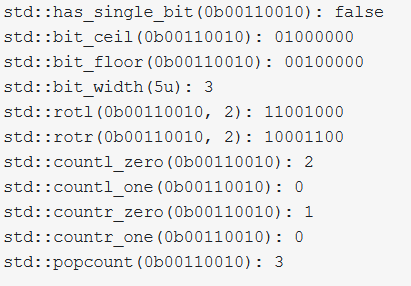
\includegraphics[width=0.6\textwidth]{content/3/chapter5/images/1-6.png}\\
Bit manipulation
\end{center}

The following program shows the std::bit\_floor, std::bit\_ceil, std::bit\_width, and std::bit\_popcount for the numbers 2 to 7.

\noindent
Displaying std::bit\_floor, std::bit\_ceil, std::bit\_width, and std::popcount for a few numbers
\begin{lstlisting}[style=styleCXX]
// bitFloorCeil.cpp

#include <bit>
#include <bitset>
#include <iostream>

int main() {
	
	std::cout << '\n';
	
	std::cout << std::boolalpha;
	
	for (auto i = 2u; i < 8u; ++i) {
		std::cout << "bit_floor(" << std::bitset<8>(i) << ") = "
		          << std::bit_floor(i) << '\n';
		
		std::cout << "bit_ceil(" << std::bitset<8>(i) << ") = "
		          << std::bit_ceil(i) << '\n';
		
		std::cout << "bit_width(" << std::bitset<8>(i) << ") = "
		          << std::bit_width(i) << '\n';
		
		std::cout << "popcount(" << std::bitset<8>(i) << ") = "
		          << std::popcount(i) << '\n';
		
		std::cout << '\n';
	}

	std::cout << '\n';
}
\end{lstlisting}

\begin{center}
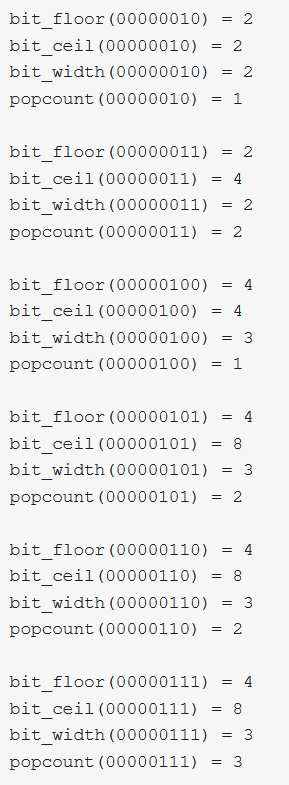
\includegraphics[width=0.4\textwidth]{content/3/chapter5/images/1-7.png}\\
Displaying std::bit\_floor, std::bit\_ceil, std::bit\_width, and std::popcount for a few numbers
\end{center}

\begin{tcolorbox}[breakable,enhanced jigsaw,colback=mygreen!5!white,colframe=mygreen!75!black,title={Distilled Information}]
	
\begin{itemize}
\item 
The cmp\_* functions in C++20 support the safe comparison of integrals because they detect the comparison of a signed and an unsigned integral. In the case of an unsafe comparison, the compilation fails.

\item 
Many mathematical constants such as $e$, $log_2e$, or $\pi$ are now defined.

\item 
C++20 provides utility functions for calculating the midpoint or linear interpolation of two values.

\item 
New functions to access and manipulate individual bits or bit sequences are available.
\end{itemize}
	
\end{tcolorbox}
\newpage